\documentclass[a4paper, 12pt]{article}
%\usepackage[T1]{fontenc}
\usepackage[left=2cm,right=2cm,top=2cm,bottom=2cm,includeheadfoot]{geometry}
\usepackage[utf8]{inputenc}
\usepackage[ngerman]{babel}
\usepackage{enumitem}
\usepackage{pdfpages}
\usepackage{ulem} 
\usepackage{graphicx}
\usepackage{caption}
\usepackage{subcaption}
\usepackage{listings}
\usepackage{verbatim}
\usepackage{fancyhdr}
\usepackage{hyperref}
\lstset{
	language=csharp,
	extendedchars=\true,
	inputencoding=utf8,
	stringstyle=\ttfamily\small, 
	showstringspaces=false,
	commentstyle=\color{codegreen},
	keywordstyle=\color{blue},
	stringstyle=\color{codegray}, 
	basicstyle=\ttfamily\small,
	breakatwhitespace=false,         
	breaklines=true, 
	captionpos=b,                    
	keepspaces=true,                 
	numbers=left,                    
	numbersep=5pt,                  
	showspaces=false,                
	showstringspaces=false,
	showtabs=false,                  
	tabsize=2,
	aboveskip=1em,
}
\usepackage{color}
\usepackage{comment}


\definecolor{codegreen}{rgb}{0,0.6,0}
\definecolor{codegray}{rgb}{0.5,0.5,0.5}
%\definecolor{backcolour}{rgb}{0.95,0.95,0.92}

\lstset{language=Java}

\pagestyle{fancy}
\lhead[Sascha Beyer, David Schneebauer]{Sascha Beyer, David Schneebauer}
\chead[Projektarbeit Hurace]{Projektarbeit Hurace}
\rhead[SWK5 GRP1 SEBakk BB WS18-19]{SWK5 GRP1 SEBakk BB WS18-19}

%opening
\title{Projektarbeit Hurace}
\author{Sascha Beyer, David Schneebauer}
\date{\today{}, Hagenberg}

\begin{document}
	\maketitle
	\tableofcontents
	\newpage
	\section{Ausbaustufe 1}
	\subsubsection{Datenbankmodell}

	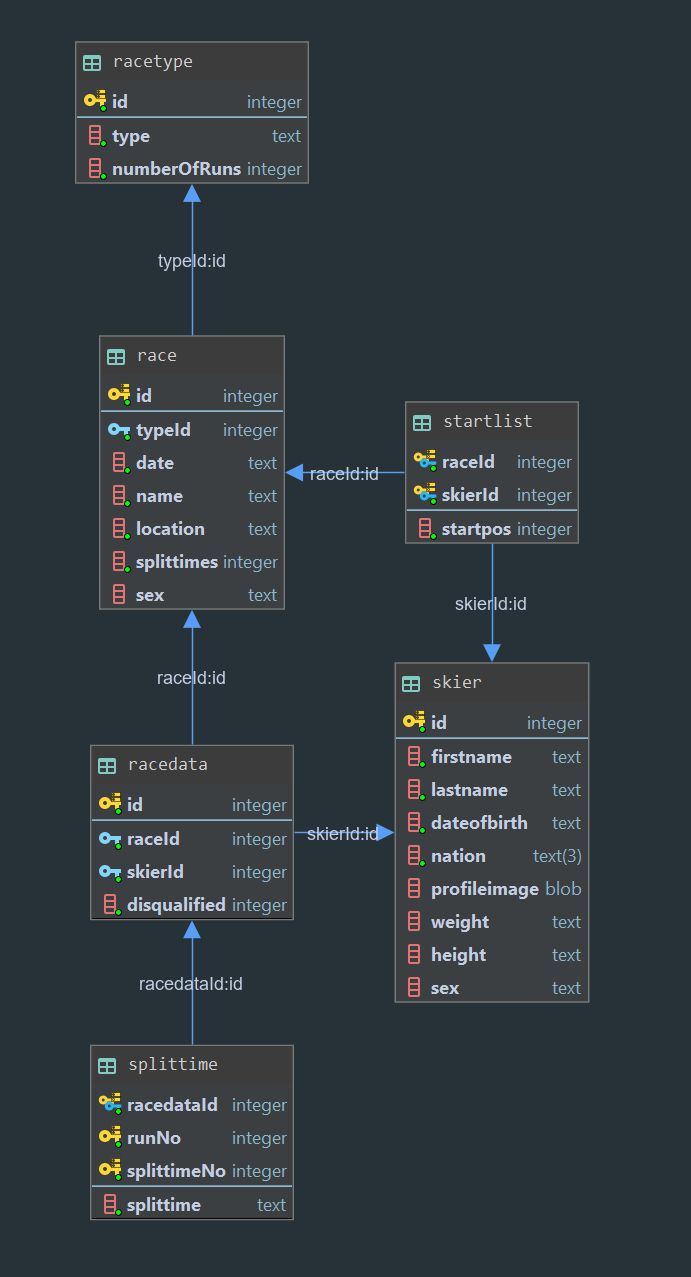
\includegraphics[width=.7\textwidth]{img/huraceDB.png}
	%\lstinputlisting[language=Java]{../src/queues/BinaryHeapQueue.java}
	%\newpage
	%\lstinputlisting[language=Java]{../src/queues/DHeapQueue.java}
	%\newpage
	\newpage
	\subsubsection{Datenbankzugriffsschicht}
	\item{IRaceDao}
	\lstinputlisting[language=csharp]{../Dal/Interface/IRaceDao.cs}
	\item{IRaceDataDao}
	\lstinputlisting[language=csharp]{../Dal/Interface/IRaceDataDao.cs}
	\item{IRaceTypeDao}
	\lstinputlisting[language=csharp]{../Dal/Interface/IRaceTypeDao.cs}
	\item{ISkierDao}
	\lstinputlisting[language=csharp]{../Dal/Interface/ISkierDao.cs}
	\item{ISplittimeDao}
	\lstinputlisting[language=csharp]{../Dal/Interface/ISplittimeDao.cs}
	\item{IStartListDao}
	\lstinputlisting[language=csharp]{../Dal/Interface/IStartListDao.cs}
	
	
	
	\newpage	
\end{document}